% template.tex, a sample LaTeX manuscript prepared for the Journal of Computer Science and Cybernetics. 
% Run LaTeX on this file twice for proper section numbers.
% A '%' causes LaTeX to ignore remaining text on the line
\input TinLatex.tex
\usepackage[utf8]{vietnam}
% \usepackage[utf8]{inputenc}
\usepackage[main=english,vietnamese]{babel}
\usepackage{subfig}
\usepackage{tabularx} % Include this package for dynamic table width
\usepackage{longtable} % Optional, if you want to use longtable

\begin{document}           % End of preamble and beginning of text.
%------------------------------------------
% Redefine "plain" pagestyl
\makeatletter	   % `@' is now a normal "letter' for LaTeX
\setcounter{page}{1}
\renewcommand{\ps@plain}{%
%\renewcommand{\@oddhead}{\small\hfill\itsl{T\ang p ch\is\ Tin h\ong c v\ah\ \DD i\eeh u khi\eehoi n h\ong c, T.25, S.1 (2009), 1--}}
\renewcommand{\@oddhead}{\hfill\begin{tabular}{r}
\small{\emph{Journal of Computer Science and Cybernetics, V.xx, N.x (20xx), 1--}} \\
\footnotesize{DOI no. 10.15625/1813-9663/xx/x/xxxx}
\end{tabular}
}

%\hfil\textrm{\thepage}}% 
    \renewcommand{\@evenhead}{\@oddhead}%
    \renewcommand{\@oddfoot}{\small\hfill{\copyright\ 20xx Vietnam  Academy of Science \& Technology}}% empty footer
    \renewcommand{\@evenfoot}{\@oddfoot}}
    \makeatother     % `@' is restored as a "non-letter" character
    

%%%%%%%%%%%%%%%%%%%%%%%%
%Title & Authors
%%%%%%%%%%%%%%%%%%%%%%%%

%=========================================================================
\title{Author guidelines for JCC submission}
\subtitle{Subtitle}
\author{
	{\cn AUTHOR NAME(S)}
	\vskip.5cm
	{\it $^1$Institute of Information Technology, Vietnam Academy of Science and Technology; \href{mailto:anonymous@ioit.ac.vn}{anonymous@ioit.ac.vn}}
	%{\it $^1$Vi\eeng n C\oo ng ngh\eeng\ th\oo ng tin, Vi\eeng n Khoa h\ong c v\ah\ C\oo ng ngh\eeng\ Vi\eeng t Nam; \href{mailto:anonymous@ioit.ac.vn}{anonymous@ioit.ac.vn}}
    \vn
    \ce{$\it NEXT AUTHOR AFFILIATION AND EMAIL ADDRESS$} 
}
%\date{}
\maketitle
\renewcommand\refname{\normalsize \centerline{ REFERENCES}}
% Set to use the "plain" pagestyle
\pagestyle{plain}
\pagestyle{myheadings}
\markboth{\footnotesize \chu  AUTHOR NAME(S)}
{\footnotesize  \chu AUTHOR GUIDELINES FOR JCC SUBMISSION }
{\cn

%=========================================================================
\begin{abstract}
This paper presents a practical, end-to-end system designed for the banking sector, enabling users to efficiently gather sentiment insights related to various aspects of banks from online sources. The system's real-world applicability lies in its ability to provide actionable sentiment analysis, which can be leveraged by banks for strategic decision-making. On the scientific front, we meticulously constructed a sentiment dataset specific to the banking industry, which was subsequently employed to evaluate the performance of various language models. This comprehensive evaluation not only demonstrates the efficacy of the dataset but also contributes valuable insights into the application of language models for sentiment analysis in the financial domain. 
\keywords{Sentiment analysis, Online Sentiment Insights, Text Mining, End-to-End Financial System, Natural Language Processing (NLP), Language Models.}
\end{abstract}

%%%%%%%%%%%%%%%%%%%%%%%%
%Main text
%%%%%%%%%%%%%%%%%%%%%%%%

%=========================================================================
\section{INTRODUCTION}

In the era of digital transformation, the banking sector is increasingly reliant on advanced technologies to understand customer sentiment and improve service delivery. This paper introduces an end-to-end system specifically designed for the banking industry, which offers a comprehensive solution for sentiment analysis. The system's practical utility lies in its ability to scrape data from various online sources, analyze sentiment, and visually represent the proportion of positive, negative, and neutral sentiments. This visualization empowers banks to gain actionable insights and make informed decisions based on customer feedback.

A core component of the system is a meticulously crafted sentiment dataset tailored for the banking domain. This dataset\footnote{Our dataset is available at \url{https://huggingface.co/datasets/iaiuet/banking_sentiment_vietnamese}} was developed using the scraped data and serves as the foundation for the sentiment analysis module. To ensure the robustness and reliability of the sentiment analysis, we evaluated the dataset using a range of language models. Specifically, we conducted inference using large language models (LLMs) such as LLama 3.1\cite{dubey2024llama3herdmodels} and Vistral\cite{chien2023vistral}, and compared their performance with fine-tuned smaller models like PhoBert\cite{phobert}, ViT5\cite{phan-etal-2022-vit5} and BartPho\cite{bartpho}.

Our findings suggest that the inherent knowledge embedded within LLMs does not significantly enhance their performance in this specific application. In contrast, the fine-tuned smaller models, when trained on the domain-specific dataset, demonstrated superior results. This observation challenges the assumption that larger models are inherently more capable and highlights the importance of domain-specific training for sentiment analysis in the financial sector.

The contributions of this paper are threefold: first, we present a highly practical system that can be readily applied in the banking industry to derive sentiment insights; second, we provide a new, domain-specific sentiment dataset for the banking sector; and third, we offer a thorough evaluation of different language models, contributing valuable knowledge to the field of natural language processing (NLP) and sentiment analysis.

%=========================================================================
\section{RELATED WORK}

All text must be in a one-column format. The main title (on the first page) should begin 1.0 inch (2.54 cm) from the top edge of the page. The second and following pages should begin 1.0 inch (2.54 cm) from the top edge. On all pages, the bottom margin should be 1-1/8 inches (2.86 cm) from the bottom edge of the page for $8.5 \times 11$-inch paper; for A4 paper, approximately 1-5/8 inches (4.13 cm) from the bottom edge of the page.

%-------------------------------------------------------------------------
\subsection{Sentiment Analysis in Banking}

All printed material, including text, illustrations, and charts, must be kept within a print area 6-7/8 inches (17.5 cm) wide by 8-7/8 inches (22.54 cm) high.

%-------------------------------------------------------------------------
\subsection{Language Models for Sentiment Analysis}

Wherever Times is specified, Times Roman may also be used. If neither is available on your word processor, please use the font closest in appearance to Times to which you have access.

%-------------------------------------------------------------------------
\subsection{Dataset Development for Sentiment Analysis}

%=========================================================================
\section{System Design and Implementation}

Our proposed system for analyzing public sentiment towards banks operates through a structured pipeline that integrates data scraping, processing, clustering, sentiment analysis, and visualization. This end-to-end approach ensures that data is systematically collected from relevant online sources, processed and stored efficiently, and then analyzed to identify sentiment trends. The final results are presented in an intuitive visual format, allowing users to easily interpret the proportions of positive, negative, and neutral sentiments. This comprehensive pipeline enhances the accuracy and practicality of sentiment analysis, making it a valuable tool for stakeholders in the banking sector.

%-------------------------------------------------------------------------
\subsection{Data Scraping}
In the data scraping phase of our system, we leverage the Scrapy framework\cite{kouzis2016learning} to extract information from various online news sources. We aim to gather data from nine distinct websites: \textit{cafef}, \textit{dantri}, \textit{kinhtedothi}, \textit{nhadautu}, \textit{vietnambiz}, \textit{vietnamnet}, \textit{vietstock}, \textit{vneconomy}, and \textit{vnexpress}.

Each website provides valuable insights into public sentiment towards banking institutions through news articles and reports. However, the available data on these websites may vary in terms of publication dates. Therefore, we establish specific timeframes for data collection from each website to ensure comprehensive coverage.

The designated timeframes for data scraping from each website are as follows:
\begin{itemize}
  \item \textbf{cafef\cite{cafef}}: Up to January 1, 2000.
  \item \textbf{dantri\cite{dantri}}: Up to approximately six months prior to the current date.
  \item \textbf{kinhtedothi\cite{kinhtedothi}}: Up to May 16, 2022.
  \item \textbf{nhadautu\cite{nhadautu}}: Up to March 25, 2017.
  \item \textbf{vietnambiz\cite{vietnambiz}}: Up to August 22, 2016.
  \item \textbf{vietnamnet\cite{vietnamnet}}: Up to September 23, 2010.
  \item \textbf{vietstock\cite{vietstock}}: Up to July 2, 2003.
  \item \textbf{vneconomy\cite{vneconomy}}: Up to July 12, 2023.
  \item \textbf{vnexpress\cite{vnexpress}}: Up to approximately six months prior to the current date.
\end{itemize}
By adhering to these timeframes, we aim to collect a diverse range of news articles spanning different periods, enabling comprehensive sentiment analysis and visualization in subsequent stages of our system.

%-------------------------------------------------------------------------
\subsection{Processing and Storing}
\subsubsection{Database Structure}

Our database is designed following the Entity-Relationship (ER) model\cite{STOREY199147}, depicted in Figure \ref{fig:er_model}. The ER model establishes relationships between entities, enhancing data integrity and facilitating complex queries. The database comprises four main tables, each serving a specific purpose:
\begin{enumerate}
    \item \textbf{SAC THAI}: This table stores paragraphs of text data along with their corresponding sentiment states and associations with banking topics. It includes the following columns:
        \begin{itemize}
            \item \textbf{id\_paragraph}: Primary key identifier for paragraphs
            \item \textbf{text\_paragraph}: Text content of the paragraph
            \item \textbf{chu\_de}: Topic of the paragraph
            \item \textbf{ngan\_hang}: Foreign key referencing the `NGAN HANG' table
            \item \textbf{sac\_thai}: the sentiment states of the paragraph
            \item \textbf{id\_ban\_tin}: Foreign key referencing the `BAN TIN' table
            \item \textbf{ngay}: Date of publication of the articles
        \end{itemize}
    \item \textbf{NGAN HANG}: This table stores information about banks, including their names and aliases. It includes the following columns:
        \begin{itemize}
            \item \textbf{id\_ngan\_hang}: Primary key identifier for banks
            \item \textbf{Ten}: Name of the bank
            \item \textbf{Ten\_viettat}: Abbreviated name of the bank
            \item \textbf{Ten\_khac}: Other aliases of the bank
        \end{itemize}
    \item \textbf{BAN TIN}: This table stores news articles related to economic topic. It includes the following columns: 
        \begin{itemize}
            \item \textbf{id\_ban\_tin}: Primary key identifier for news articles
            \item \textbf{Nguon}: Source of the news article
            \item \textbf{Ngay}: Date of publication
            \item \textbf{text}: Text content of the news article
            \item \textbf{url}: URL of the news article
            \item \textbf{url\_hash}: Hash value of the URL
        \end{itemize}
    \item \textbf{CHU DE}: This table stores information about topics, including their names and synonyms. It includes the following columns:
        \begin{itemize}
            \item \textbf{id\_chu\_de}: Primary key identifier for topics
            \item \textbf{Ten}: Name of the topic
            \item \textbf{Dong\_nghia}: Synonyms of the topic
            \item \textbf{Tich\_cuc}: Keywords for positive sentiments about the topic
            \item \textbf{Tieu\_cuc}: Keywords for negative sentiments about the topic
            \item \textbf{id\_chu\_de\_con}: Identifier for subtopics
        \end{itemize}
\end{enumerate}

\begin{figure}[t]
  \begin{center}
  \fbox{\rule{0pt}{2in} 
      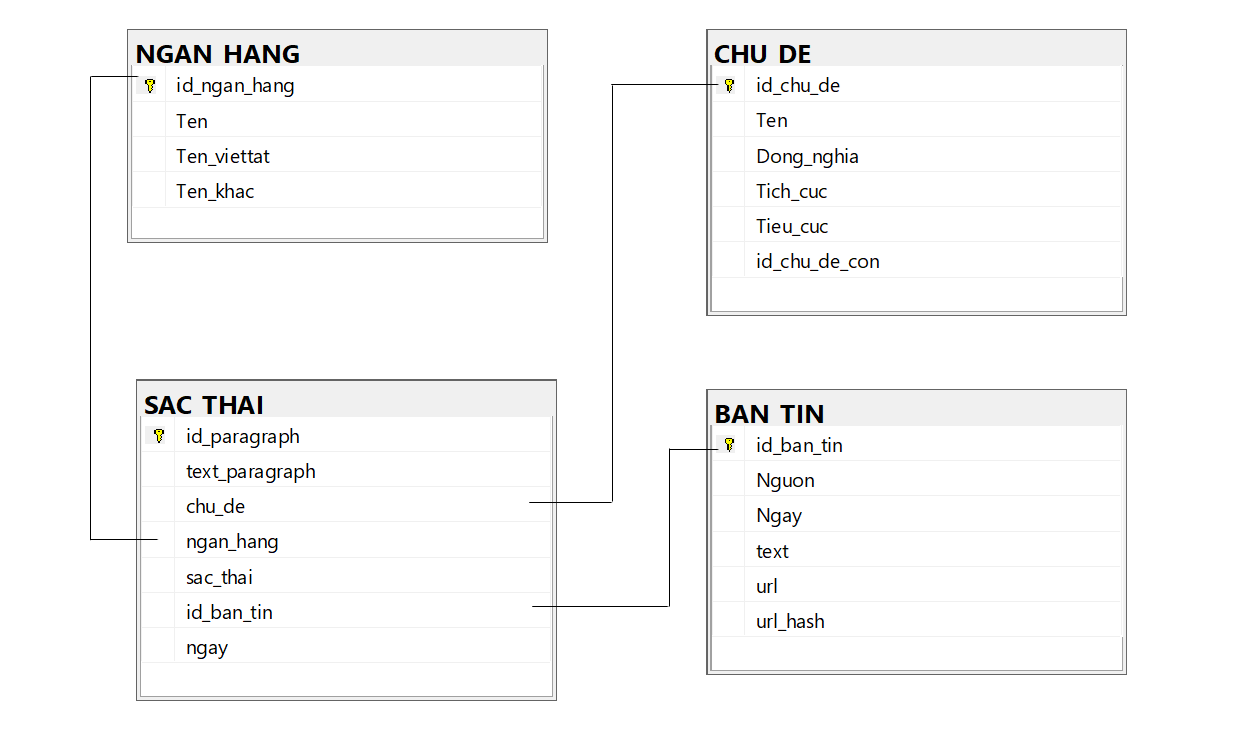
\includegraphics[width=0.95\linewidth]{images/diagram.png}
  }
  \end{center}
  \caption{\small Database diagram}
\label{fig:er_model}%
\end{figure}

\subsubsection{Data Classification}
Upon retrieval, the text data undergoes NLP-based classification to identify its relevance to economic topics. The module use standard binary-classification pipeline: feature extraction with TF-IDF (Term Frequency-Inverse Document Frequency), and classify using SVM (Support Vector Machine). This classification step ensures that only economically significant data is further processed and analyzed. The performance of this classification model was evaluated using a test set, and the results are shown in Table \ref{tab:Classifier result}. Subsequently, the economically relevant data is stored in the `BAN TIN' table for further analysis.

\begin{table}
  \begin{center}
    \begin{tabular}{|l|l|l|l|l|}
      \hline
       & \textbf{precision} & \textbf{recall} & \textbf{f1-score} &\textbf{support}  \\ 
      \hline Not Economic-Related  & 0.76 & 0.80 & 0.78 & 188  \\ 
      \hline Economic-Related & 0.81 & 0.78 & 0.80 & 212 \\ 
      \hline accuracy  &  &  & 0.79 & 400 \\
      \hline macro avg  & 0.79 & 0.79 & 0.79 & 400 \\
      \hline weighted avg  & 0.79 & 0.79 & 0.79 & 400 \\
      \hline
    \end{tabular}%
  \end{center}
  \caption{\small Performance of the SVM Classifier with TF-IDF.}
  \label{tab:Classifier result}
\end{table}

%-------------------------------------------------------------------------
\subsection{Clustering and Segmenting}
Within the Clustering and Segmenting phase, our system employs sophisticated algorithms to segment news articles retrieved from the `BAN TIN' table within the database. The objective is to extract segments discussing specific banks within a given topic, enhancing the precision and relevance of subsequent analysis. The workflow of this module unfolds as follows:

\subsubsection{Text Segmentation}
The module retrieves news articles from the `BAN TIN' table in the database, then initiates the process of text segmentation. This involves breaking down the article into smaller segments, each representing a coherent and meaningful unit of information. By segmenting the text, the module ensures that fine-grained analysis can be conducted on specific aspects of the content

\subsubsection{Topic Identification}
Concurrently, the module discerns the overarching topic(s) discussed within each article by leveraging keyword extraction techniques. This process involves extracting relevant keywords from the text, utilizing a predefined list of topics stored in the `CHU DE' table within the database. By matching keywords extracted from the article with those in the topic repository, the module identifies the primary themes and subtopics addressed in the text. This approach enables efficient topic identification without relying on complex topic modeling algorithms, ensuring timely and accurate classification of articles based on predefined topic categories

\subsubsection{Bank Entity Recognition}
In this process, the module employs name-based recognition techniques, drawing upon data from the `NGAN HANG' table stored in the database. By extracting bank names, abbreviations, and other aliases from the database, the module accurately identifies mentions of specific banks within each segmented article. This approach ensures precise recognition of bank entities in the text, facilitating comprehensive analysis of banking-related discussions without the need for complex models

\subsubsection{Segment Filtering}
Subsequently, the module filters the segmented text to retain only those segments that pertain to specific banks within the identified topic(s). This filtering process ensures that subsequent analysis is focused on relevant discussions related to the banking sector. The retained segments are then passed on to the next module for sentiment analysis, as discussed in subsequent sections. This sequential workflow ensures that only pertinent segments contribute to the sentiment analysis process, enhancing the accuracy and relevance of the insights generated.

%-------------------------------------------------------------------------
\subsection{Sentiment Analysis}

Our sentiment analysis module leverages two advanced models: Vistral and PhoBERT, known for their exceptional accuracy and robustness in processing textual sentiment, particularly in Vietnamese.
\begin{itemize}
    \item \textbf{Vistral}: Vistral is a multi-turn conversational large language model for Vietnamese. Vistral is extended from the Mistral 7B model using diverse data for continual pre-training and instruction tuning.
    \item \textbf{PhoBERT}: PhoBERT is built upon the powerful BERT (Bidirectional Encoder Representations from Transformers) framework, is the first public large-scale monolingual language models pre-trained for Vietnamese. It boasts remarkable capabilities in multiple Vietnamese-specific NLP tasks including Part-of-speech tagging, Dependency parsing, Named-entity recognition and Natural language inference.
\end{itemize}

Details on the performance of these models are provided in the following sections.

After sentiment analysis, the processed paragraphs are stored in the `SAC THAI' table along with their corresponding sentiments.\par
By integrating Vistral and PhoBERT into our sentiment analysis module and storing the results in the database, our system ensures accurate sentiment classification, enabling comprehensive analysis of textual data within the financial domain.

%-------------------------------------------------------------------------
\subsection{Visualization}

\begin{figure}[t]
  \begin{center}
  \fbox{\rule{0pt}{2in} 
      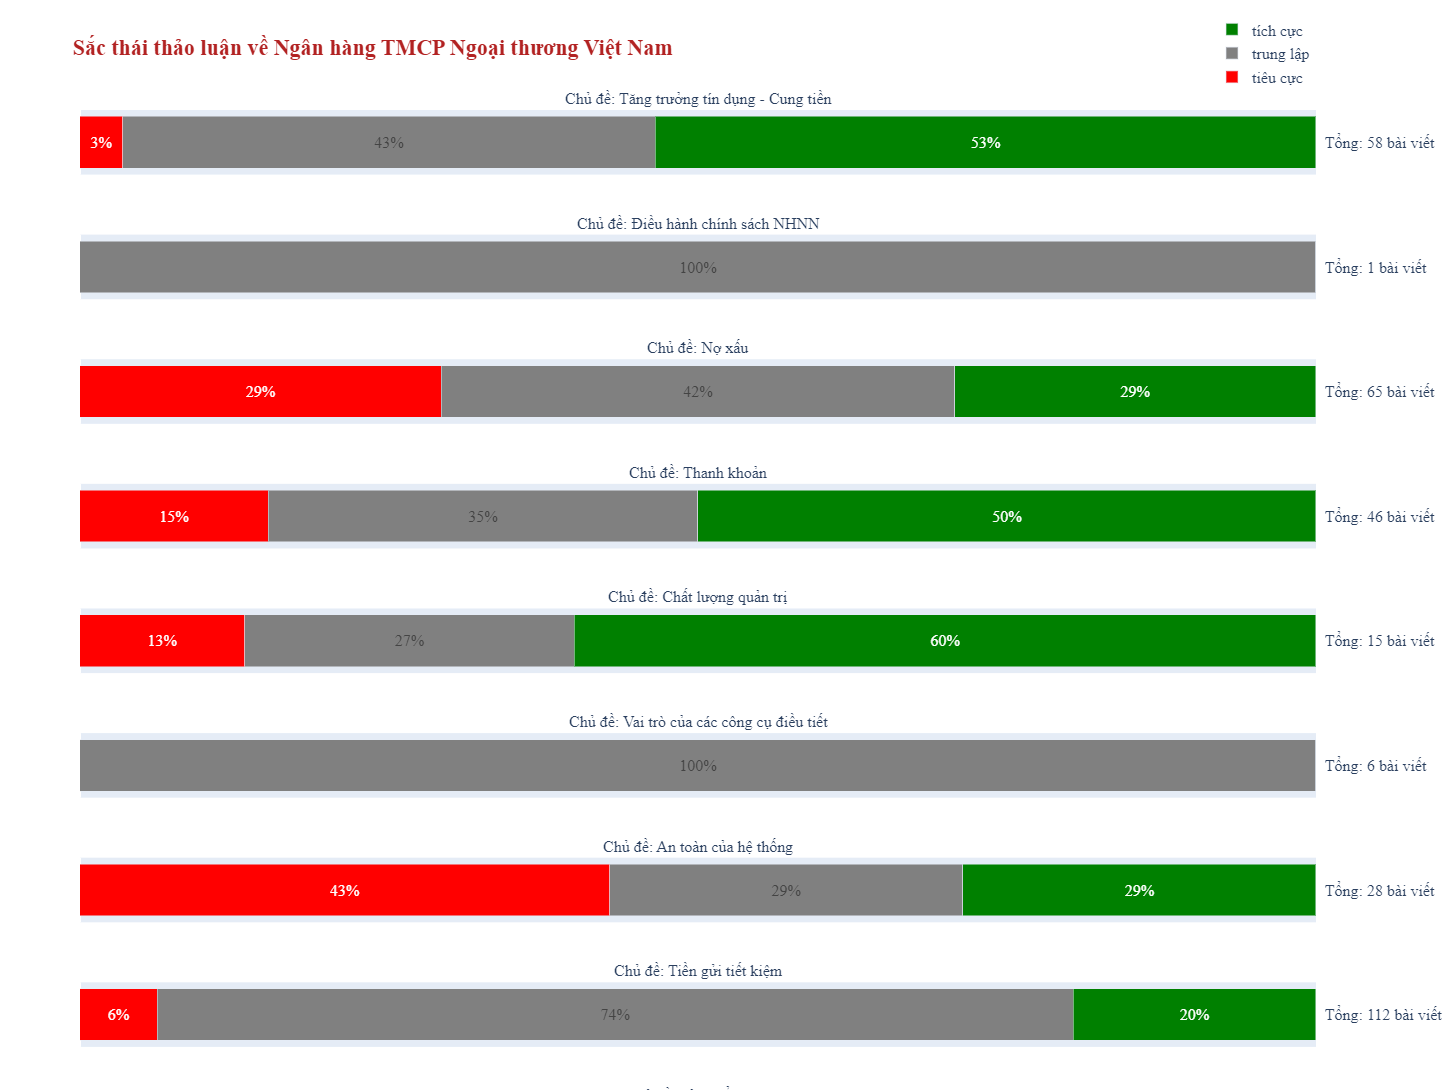
\includegraphics[width=0.95\linewidth]{images/newplot.png}
  }
  \end{center}
  \caption{\small Distribution of sentiment (positive, negative, neutral) across various banks during a specific quarter, highlighting the public perception of each bank's performance.}
\label{fig:bank_dist}%
\end{figure}

Our system employs sophisticated data visualization techniques to transform processed sentiment data into interactive and insightful charts and graphs. The visualization process begins by extracting relevant data from the `SAC THAI' table in the database. This data is then filtered based on the desired criteria, such as specific banks, topics, and time periods. Once filtered, the sentiment scores (positive, negative, and neutral) are aggregated for each bank, topic, and time period to facilitate comprehensive trend analysis. \par
To create these visualizations, we utilize the advanced data visualization library Matplotlib\cite{Hunter:2007}. Our system supports various types of charts, including bar charts and pie charts, Our system supports many different chart types, including bar charts and pie charts, in this report, stacked bar charts will be taken as an example. This chart effectively illustrates the distribution of sentiment across different categories. As shown in Figure \ref{fig:bank_dist}, the stacked bar chart includes the following elements: the X-axis represents categories such as banks, topics, or time periods, while the Y-axis shows the percentage of sentiment (positive, negative, neutral). Each stacked bar represents the proportion of each sentiment category, with a legend indicating the different sentiment types. Tooltips are incorporated to provide detailed information about each data point, enhancing user understanding and engagement. \par
The system is designed to be highly interactive, allowing users to filter the data by selecting specific banks, topics, or time periods. Users can also drill down to view sentiment distribution at a more granular level, such as individual articles or specific dates. Hover effects are implemented to display additional information when users hover over data points, offering deeper insights into the sentiment data. \par

Customization options are available to users, enabling them to adjust the appearance of the charts, including colors, fonts, and styles. Additionally, the system provides options to export the charts in various formats, such as PNG, JPEG, or PDF, for reporting and presentation purposes. Users can also export the underlying data in Excel (xlsx) format, allowing for further analysis using tools like Excel or PowerBI.\par

%=========================================================================
\section{DATASET DEVELOPMENT}

To effectively analyze sentiment in the banking sector, we developed a comprehensive dataset using the aforementioned system. The dataset consists of 10,000 training samples and 2,000 test samples, all collected through our end-to-end system that scrapes relevant online data. The data was carefully labeled by human annotators, with each sample categorized into one of three sentiment labels: positive, negative or neutral.

The dataset covers a wide range of topics, spanning 13 key aspects of the banking industry. These topics include: Bank Capital, Credit Growth - Money Supply, Role of Regulatory Tools, Savings Deposits, Liquidity, Banking Services, State Bank Policy Implementation, Management Quality, Non-Performing Loans (NPLs), Digitalization of Banking Operations, Loan Products, Business Efficiency and System Safety.

Given the diverse nature of these topics, the dataset provides a well-rounded view of sentiment across different facets of banking. The data is entirely in Vietnamese, reflecting the language used in the source material. The distribution of data across these 13 topics is summarized in the table \ref{tab:topic_distribution}.

\begin{table}
  \begin{center}
    \begin{tabular}{|l|l|l|}
      \hline
       & \textbf{train} & \textbf{test}  \\ 
      \hline Bank Capital  & 846 & 168 \\ 
      \hline Credit Growth - Money Supply & 1198 & 212 \\ 
      \hline Role of Regulatory Tools  & 292 & 67  \\
      \hline Savings Deposits  & 793 & 142  \\
      \hline Liquidity  & 949 & 196  \\
      \hline Banking Services  & 1495 & 311  \\
      \hline State Bank Policy Implementation  & 255 & 60  \\
      \hline Management Quality  & 390 & 72  \\
      \hline Non-Performing Loans  & 1381 & 286  \\
      \hline Digitalization of Banking Operations  & 859 & 146  \\
      \hline Loan Products  & 554 & 124  \\
      \hline Business Efficiency  & 635 & 134  \\
      \hline System Safety  & 353 & 82  \\
      \hline
    \end{tabular}%
  \end{center}
  \caption{\small Distribution of data across different topics in the dataset.}
  \label{tab:topic_distribution}
\end{table}

This dataset is meticulously designed for sentiment analysis within the banking sector, offering deep insights into public opinion across a broad spectrum of banking topics. By covering 13 distinct aspects of the banking industry, the dataset provides a highly practical and comprehensive foundation for training and evaluating sentiment analysis models. Its extensive coverage ensures that the models are well-aligned with the diverse and nuanced realities of the financial domain, making the dataset exceptionally relevant for real-world applications. Some examples of the dataset are shown in Appendix \ref{app:dataset}

%=========================================================================
\section{EXPERIMENTAL SETUP}
To evaluate the effectiveness of sentiment analysis in the banking domain, we conducted a series of experiments using both large language models (LLMs) and smaller, fine-tuned models. The LLMs, specifically LLama 3.1 and Vistral, were used exclusively for inference without any fine-tuning. We explored their performance across a range of prompts designed to reflect various aspects of sentiment analysis.

The inference was performed using the following types of prompts:
\begin{itemize}
  \item\textbf{Zero-shot without External Knowledge}: Prompts were provided without any additional context or definitions related to what constitutes positive, negative, or neutral sentiment.
  \item\textbf{Zero-shot with External Knowledge}: Prompts included additional context, explicitly defining what constitutes positive, negative, and neutral sentiment to guide the models.
  \item\textbf{Few-shot without External Knowledge}: Prompts included 1 to 5 examples but did not provide additional context or definitions.
  \item\textbf{Few-shot with External Knowledge}: Prompts included 1 to 5 examples along with definitions of sentiment categories, offering more guidance to the models.
\end{itemize}

For the few-shot prompts, we retrieved relevant documents from the training set that belonged to the same topic using a vector database implemented with Faiss\cite{douze2024faiss}.

In contrast, smaller models such as BARTPho, PhoBERT, and ViT5 were fine-tuned on our domain-specific dataset to optimize their performance in sentiment analysis. These models underwent training on the dataset with the goal of capturing the nuanced sentiment expressed across the 13 topics within the banking sector.

All models, both LLMs and smaller models, were trained and inferred using a V100 16GB GPU. This setup allowed us to compare the out-of-the-box performance of large language models with the fine-tuned performance of smaller models, providing insights into the impact of model size, training, and the inclusion of external knowledge on sentiment analysis accuracy.

%=========================================================================
\section{RESULTS AND DISCUSSION}
\begin{table}[htbp]
  \small
  \setlength{\tabcolsep}{2pt} % Adjust column spacing
  \begin{center}
    \begin{tabular}{|l|c|l|c|c|}
      \hline
      & \textbf{Prompt Type} & \textbf{Acc.} & \textbf{Inference Time} &\textbf{GPU Usage}  \\ 
       &  &  & \textbf{(minutes)} & \textbf{(GB)} \\ 
      \hline LLama 3.1 (quant.) & 0-shot, No external knowledge & 0.551 & 24 & 7.816 \\ 
      \hline LLama 3.1 (quant.) & 1-shot, No external knowledge	 & 0.5265 & 30 & 8.148 \\ 
      \hline LLama 3.1 (quant.) & 2-shot, No external knowledge	 & 0.567 & 32.6 & 8.424\\
      \hline LLama 3.1 (quant.) & 3-shot, No external knowledge	 & 0.587 & 35.5 & 8.844\\
      \hline LLama 3.1 (quant.) & 4-shot, No external knowledge	 & 0.595 & 36.7 & 9.158\\
      \hline LLama 3.1 (quant.) & 5-shot, No external knowledge	 & \textbf{0.6175} & 39.5 & 9.414\\
      \hline LLama 3.1 (quant.) & 0-shot, With external knowledge & 0.4635 & 25.5 & 7.838\\ 
      \hline LLama 3.1 (quant.) & 1-shot, With external knowledge	 & 0.4985 & 31.6 & 8.172\\ 
      \hline LLama 3.1 (quant.) & 2-shot, With external knowledge	 & 0.525 & 37 & 8.41\\
      \hline LLama 3.1 (quant.) & 3-shot, With external knowledge	 & 0.555 & 37.9 & 8.902\\
      \hline LLama 3.1 (quant.) & 4-shot, With external knowledge	 & 0.5725 & 40.7 & 9.256\\
      \hline LLama 3.1 (quant.) & 5-shot, With external knowledge	 & 0.5665 & 41 & 9.492\\
      \hline Vistral (quant.)  & 0-shot, No external knowledge & 0.5375 & 28.7 & 6.738\\
      \hline Vistral (quant.)  & 1-shot, No external knowledge & 0.354 & 45.8 & 6.816\\
      \hline Vistral (quant.)  & 2-shot, No external knowledge & 0.354 & 57 & 9.053\\
      \hline Vistral (quant.)  & 3-shot, No external knowledge & 0.4 & 68.8 & 9.443\\
      \hline Vistral (quant.)  & 4-shot, No external knowledge & 0.4335 & 81.2 & 8.33\\
      \hline Vistral (quant.)  & 5-shot, No external knowledge & 0.4845 & 97 & 11.97\\
      \hline Vistral (quant.)  & 0-shot, With external knowledge & 0.529 & 39 & 7.287\\
      \hline Vistral (quant.)  & 1-shot, With external knowledge & 0.4105 & 66 & 7.104\\
      \hline Vistral (quant.)  & 2-shot, With external knowledge & 0.3715 & 78 & 10.484\\
      \hline Vistral (quant.)  & 3-shot, With external knowledge & 0.4095 & 78 & 9.67\\
      \hline Vistral (quant.)  & 4-shot, With external knowledge & 0.435 & 92 & 11.184\\
      \hline Vistral (quant.)  & 5-shot, With external knowledge & 0.48 & 105.8 & 12.268\\
      \hline PhoBERT (fine-tuned)  &  & 0.689 & 0.50 & 0.214\\
      \hline BARTPho (fine-tuned) &  & 0.678 & 0.77 & 0.889\\
      \hline ViT5 (fine-tuned)  &  & 0.682 & 1.45 & 1.482\\
      \hline
    \end{tabular}%
  \end{center}
  \caption{\small Performance comparison of sentiment analysis models in terms of accuracy, GPU usage, and inference time across different prompt configurations.} 
  \label{tab:results}
\end{table}

The performance of the sentiment analysis models was evaluated using accuracy as the primary metric, alongside considerations of GPU usage and inference time. Our experiments reveal several noteworthy trends, as detailed below.

First, the fine-tuned smaller models BARTPho\footnote{Our model is available at \url{https://huggingface.co/iaiuet/bartpho-banking-sentiment}}, PhoBERT\footnote{Our model is available at \url{https://huggingface.co/iaiuet/PhoBERT-base-sentiment}}, and ViT5\footnote{Our model is available at \url{https://huggingface.co/iaiuet/vit5-base_sentiment}} consistently outperformed the larger language models (LLMs) such as LLama 3.1 and Vistral when it came to accuracy. Despite their smaller size, these models not only achieved higher accuracy but also required significantly less computational resources and ran much faster, demonstrating the efficiency and effectiveness of fine-tuning in specialized domains like banking.

For the LLMs, accuracy improved as more shots were provided during inference. The highest accuracy was achieved by the quantized version of LLama 3.1 using a 5-shot prompt without external knowledge, reaching an accuracy of 0.6175. However, this came at the cost of higher GPU usage and longer inference times compared to the smaller models. In term of large language models, LLama 3.1 generally showed higher accuracy, used less GPU memory, and completed inference faster compared to Vistral. This indicates that LLama 3.1 is more efficient and better suited for sentiment analysis in this context, particularly when GPU resources and inference time are constrained.

An unexpected finding was the decrease in accuracy when external knowledge was introduced in the prompts. Contrary to expectations, this additional context led to lower performance across all LLM configurations. This suggests that the inclusion of external knowledge may introduce noise or confusion rather than improving model understanding, a phenomenon that warrants further investigation.

From these results, it is evident that the inherent knowledge of LLMs does not always translate into better performance. This outcome indicates that LLMs' pre-existing knowledge may not be entirely effective or even beneficial in specific sentiment analysis tasks, particularly in the nuanced context of banking.

Table \ref{tab:results} summarizes the accuracy, GPU usage, and inference time for different models and prompt configurations, all conducted on the V100 16GB GPU.

In summary, while LLMs show promise with few-shot learning, our results underscore the advantages of fine-tuning smaller models, particularly in terms of accuracy, resource efficiency, and speed. The unexpected drop in accuracy with external knowledge prompts indicates a need for further research to better understand and optimize the use of LLMs in sentiment analysis.

%=========================================================================
\section{CONCLUSION AND FUTURE WORK}
\subsection{Summary of Contributions}
In this paper, we presented a comprehensive end-to-end system for sentiment analysis within the banking sector, leveraging a combination of large language models (LLMs) and smaller, fine-tuned models. Our system's ability to scrape data, perform sentiment analysis, and visualize results makes it a valuable tool for understanding public sentiment on a wide range of banking topics.

The newly developed sentiment analysis dataset, specifically tailored for the banking domain and covering 13 distinct topics, serves as a critical resource for training and evaluating sentiment models. Our experiments demonstrated that smaller, fine-tuned models like BARTPho, PhoBERT, and ViT5 outperform larger LLMs such as LLama 3.1 and Vistral in terms of accuracy, resource efficiency, and inference speed. This outcome highlights the practical advantages of domain-specific fine-tuning over relying solely on the extensive pre-existing knowledge within LLMs.

Interestingly, our results also revealed that providing LLMs with external knowledge did not enhance their performance as expected, sometimes even leading to a decline in accuracy. This suggests that LLMs'inherent knowledge, while extensive, may not always align with the specific nuances of domain-specific tasks like sentiment analysis in banking.

In conclusion, while LLMs offer powerful capabilities, our findings suggest that for specialized tasks within constrained environments, smaller, fine-tuned models may offer more reliable and efficient performance. Future work could explore the factors contributing to the observed inefficacy of external knowledge in LLMs and seek to optimize their application in specialized domains.

\subsection{Future Work}
Future work will focus on improving the data classification process within the Processing and Storing module. This improvement will involve refining algorithms and methodologies to better categorize economic content, thereby increasing the relevance and accuracy of sentiment analysis.

%=========================================================================
\section*{APPENDIX}

\appendix
\subsection{Example of the dataset}\label{app:dataset}
Table \ref{tab:dataset_examples} illustrate the structure and content of our sentiment analysis dataset, which is specifically tailored for the banking sector. The dataset consists of sentences labeled as positive, negative, or neutral, each covering various banking topics such as bank capital, credit growth, digitalization of banking operations...

\begin{table}[h!]
  \begin{center}
  \begin{tabularx}{\textwidth}{|p{4cm}|X|l|}
  \hline
  \textbf{Topic} & \textbf{Text} & \textbf{Label} \\
  \hline
  \textbf{Bank Capital} & Tăng vốn điều lệ, từng bước nâng tầm vị thế
  VPB đã có một nhịp tăng ấn tượng bắt đầu từ tháng 04/2020. Trong đó, điểm nhấn là giai đoạn bắt đầu từ tháng 02/2021 đến tháng 06/2021 khi cổ phiếu này liên tục phá đỉnh, tăng hơn 150\% từ mức giá 28,000 lên hơn 70,000 sau khi đón nhận nhiều thông tin tích cực từ kết quả kinh doanh, bán 49\% cổ phần FE Credit, tăng vốn điều lệ “khủng”
  (\textit{Increasing charter capital, progressively elevating the status
  VPB has experienced an impressive growth trajectory starting from April 2020. Notably, from February 2021 to June 2021, the stock consistently reached new highs, increasing more than 150\% from a price of 28,000 to over 70,000 after receiving positive news including business results, the sale of a 49\% stake in FE Credit, and a significant increase in charter capital.}). & Positive \\
  \hline
  \textbf{Credit Growth - Money Supply} & Các doanh nghiệp phi tài chính như thép, phân bón, dầu khí, bán lẻ, xây dựng, hóa chất, du lịch... đều tăng trưởng âm, thậm chí thua lỗ nặng trong quý cuối năm 2022. Kết quả kinh doanh của nhóm bất động sản cũng không mấy khả quan trước khó khăn bởi 2 kênh huy động vốn chủ yếu là tín dụng ngân hàng và trái phiếu bị thắt chặt. 
  (\textit{Non-financial businesses such as steel, fertilizers, oil and gas, retail, construction, chemicals, and tourism all experienced negative growth, and even incurred heavy losses in the last quarter of 2022. The financial performance of the real estate sector was also not very promising due to difficulties, as the two main funding channels—bank credit and bonds—were tightened.}) & Negative \\
  \hline
  \textbf{Banking Services} & Ở giai đoạn 2 đến hết ngày 11/08/2024, với hai kỳ xét giải, chủ thẻ tín dụng Sacombank Visa hạng Infinite/Signature/Platinum có cơ hội được hoàn tiền đến 2 triệu VND . Theo đó, 1,000 khách hàng có doanh số giao dịch thẻ tại nước ngoài cao nhất (tối thiểu từ 4 triệu VND ) sẽ được hoàn 1 triệu VND/kỳ. 
  (\textit{In Phase 2, until August 11, 2024, with two evaluation periods, Sacombank Visa Infinite/Signature/Platinum credit cardholders have the opportunity to receive a cashback of up to 2 million VND. Accordingly, the top 1,000 customers with the highest transaction volume abroad (minimum of 4 million VND) will receive a cashback of 1 million VND per period.})& Neutral \\
  \hline
  \end{tabularx}
\end{center}
  \caption{Examples from the sentiment analysis dataset, showcasing various banking topics with their corresponding sentiment labels.}
  \label{tab:dataset_examples}
\end{table}

These examples reflect the diversity and specificity of the topics covered in the dataset, enabling accurate sentiment analysis across a wide range of banking-related issues.

%=========================================================================
\section*{ACKNOWLEDGMENT}

The preferred spelling of the word ``acknowledgment'' in American English is without an ``e'' after the ``g.'' Use the singular heading even if you have many acknowledgments. Avoid expressions such as ``One of us (S.B.A.) would like to thank ... .'' Instead, write ``F. A. Author thanks ... .'' In most cases, sponsor and financial support acknowledgments are placed in the unnumbered footnote on the first page, not here.



%=========================================================================
% References

% BibTeX users please use
{\small
\bibliographystyle{IEEEtranS} % sorted IEEE style
\bibliography{template} % name your BibTeX data base
}

\hfill {\it Received on September 01 - 2024}

\hfill {\it Revised on October 14 - 2024}
\end{document}
